% ### Uses XeLaTeX ### %
% ### Needs beamer-master ### %
\documentclass[aspectratio=169]{beamer} %. Aspect Ratio 16:9
\usetheme{AI2} % beamerthemeSprace.sty
% DATA FOR FOOTER
\date{2019}
\title{}
\author{}
\institute{Advanced Institute for Artificial Intelligence (AI2)}
\begin{document}    
% ####################################
% FIRST SLIDE 						:: \SliTit{<Title of the Talk>}{<Author Name>}{<Intitution>}
% SLIDE SUB-TITLE					:: \SliSubTit{<Title of the Chapter>}{<Title of the Section>}
% SLIDE WITH TITLE 					:: \SliT{<Title>}{Content}
% SLIDE NO TITLE 						:: \Sli{<Content>} 
% SLIDE DOUBLE COLUMN WITH TITLE 	:: \SliDT{<Title>}{<First Column>}{<Second Column>}
% SLIDE DOUBLE COLUMN NO TITLE 		:: \SliD{<First Column>}{<Second Column>}
% SLIDE ADVANCED WITH TITLE 			:: \SliAdvT{<Title>}{<Content>}
% SLIDE ADVANCED  NO TITLE 			:: \SliAdv{<Content>}
% SLIDE ADVANCED DOUBLE TITLE 		:: SliAdvDT{<Title>}{<First Column>}{<Second Column>}
% SLIDE ADVANCED DOUBLE NO TITLE 	:: SliAdvD{<First Column>}{<Second Column>}
% ITEMIZE 							:: \begin{itemize}  \IteOne{1st Level} \IteTwo {2nd Level} \IteThr{3rd Level} \end{itemize}
% SECTION 							:: \secx{Section} | \secxx{Sub-Section}
% COLOR BOX 						:: \blu{blue} + \red{red} + \yel{yellow} + \gre{green}
% FRAME 							:: \fra{sprace} \frab{blue} \frar{red} + \fray{yellow} + \frag{green}	
% REFERENCE						:: \refer{<doi number>}
% FIGURE 							::  \img{X}{Y}{<scale>}{Figures/.png} 
% FIGURE							:: \begin{center}\includegraphics[scale=<#>]{Figures/.png}\end{center}
% PROJECT STATUS					:: \planned\~    \started\~   \underway\~   \done\~   
% EXERCICIO							:: \Exe{<#>}{<text>}
% STACKREL							:: \underset{<down>}{<up>}
% FLUSH LEFT						:: \begin{flalign*}  & <1st equation> & \\  & <12nd equation>  & \\ \end{flalign*}
% REAL / IMAGINAY					:: \Re / \Im
% SLASH								:: \sl{} or \sl
% BOLD MATH							:: \pmb{<>}
% ####################################
%
% FIRST SLIDE :: DO NOT BREAK LINE !!!
\SliTit{Git}{Advanced Institute for Artificial Intelligence}{https://advancedinstitute.ai}

% SLIDE WITH TITLE
\SliT{Sumário}{

\begin{itemize}
    \IteOne{Conceitos}
    \IteOne{Comandos}
    \IteOne{Github}
    \IteOne{Fluxos para Gerenciamento de Código}
 \end{itemize}

}

\SliT{Git}{

Características elementares do Git

\begin{itemize}
    \IteOne{É um sistema de controle de versão de arquivos que rastreia o histórico de mudanças à medida que pessoas e equipes colaboram nos projetos juntos. }
    \IteOne{ Provê mecanismos para tornar mais controlado o processo de executar testes, corrigir erros e contribuir com novos fragmentos de código}
    \IteOne{ Permite recuperar quaiquer versões anteriores}
\end{itemize}

}

\SliT{Git}{

Características elementares do Git

\begin{itemize}
    \IteOne{Provê um controle de versionamento completamente distribuído.}
    \IteOne{Não precisa de uma conexão constante com um repositório central, assim os desenvolvedores podem trabalhar em qualquer lugar e colaborar de forma assíncrona}
    \IteOne{Permite gerenciar as alterações localmente, antes de enviar para uma instância remota}
    \IteOne{Inicialmente projetado para fazer o controle de versão no kernel do Linux, mas na prática é uma das ferramentas mais utilizadas para desenvolvimento colaborativo de software }

\end{itemize}

}

\SliT{Git}{

\begin{center}
    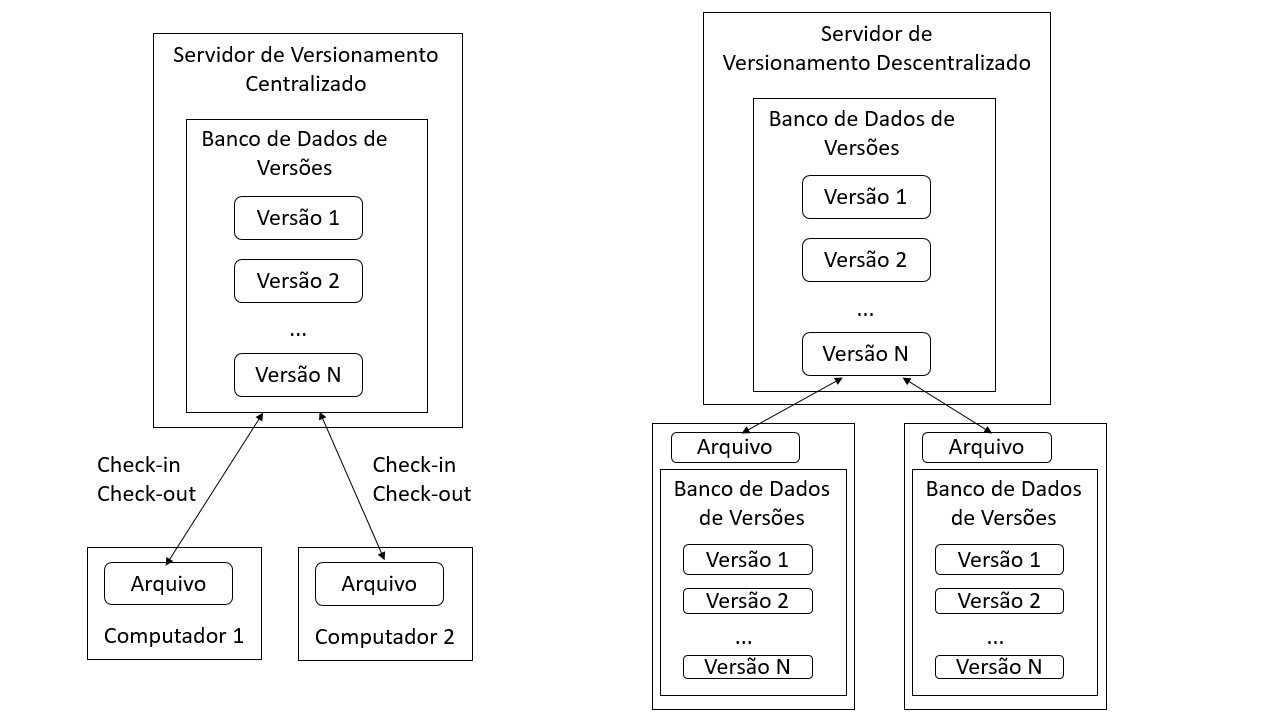
\includegraphics[scale=0.35]{img/Slide3.jpg}     
    \end{center}
}



\SliT{Comandos Git}{

\begin{itemize}
      \IteOne{git init inicializa um novo repositório Git e começa a rastrear um diretório existente.} 

      \IteOne{git add (arquivo) controla as alterações de um arquivo no repositório local} 

      \IteOne{git commit salva o snaphsot no histórico do projeto e conclui o processo de controle de alterações. }

      \IteOne{git status  mostra o status das alterações como não rastreadas, modificadas ou preparadas.}

      \IteOne{git push atualiza o repositório remoto com quaisquer confirmações feitas localmente em uma branch.}
      
\end{itemize}

}

\SliT{Comandos Git}{

\begin{center}
    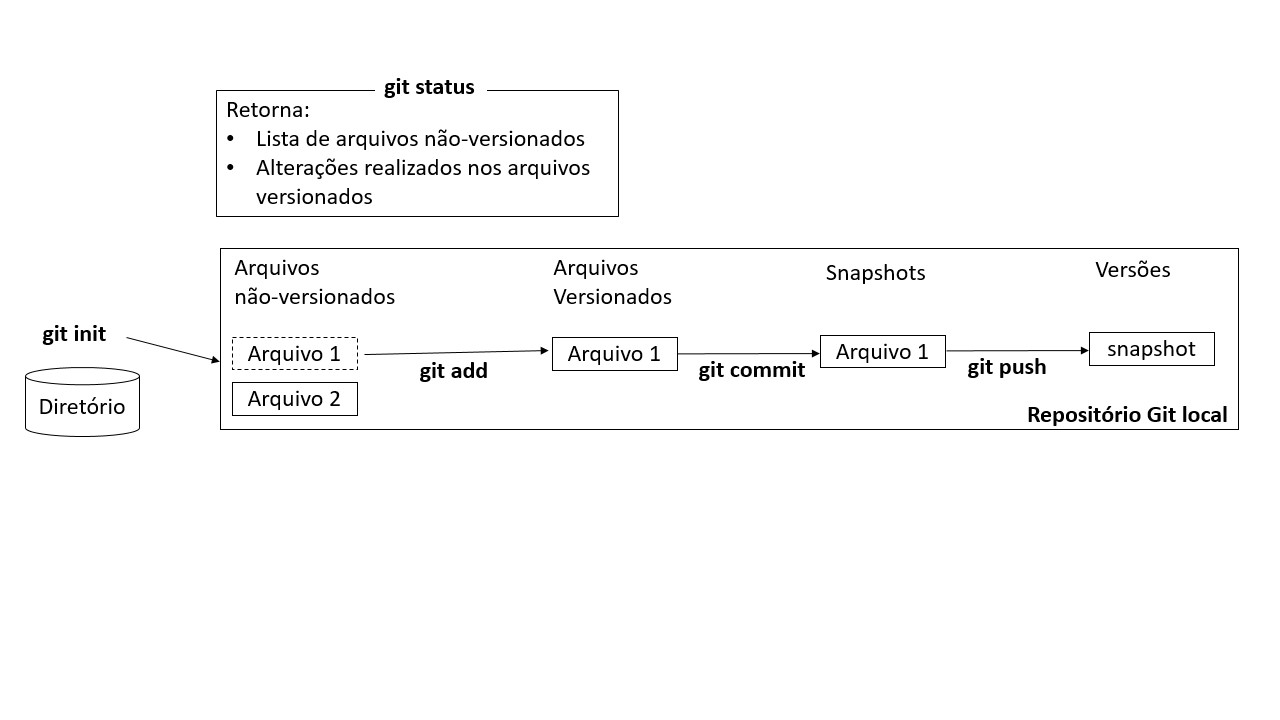
\includegraphics[scale=0.35]{img/git11.jpg}     
    \end{center}
}

\SliT{Comandos Git}{

\begin{itemize}

      \IteOne{git clone cria uma cópia local de um projeto que já existe remotamente. O clone inclui todos os arquivos, histórico e branches do projeto.}

    \IteOne{git pull atualiza o repositório local com atualizações do repositório remoto. }
      
\end{itemize}

\begin{center}
    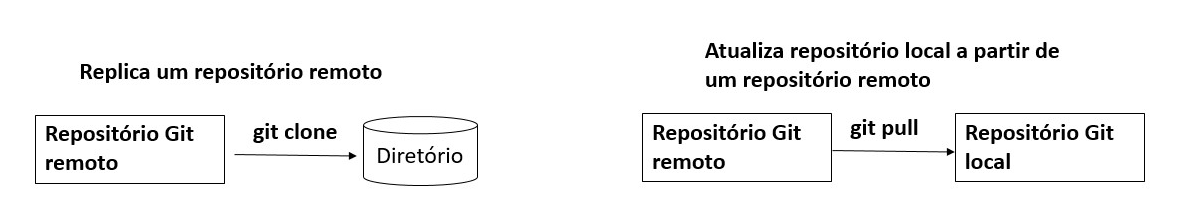
\includegraphics[scale=0.35]{img/git21.png}     
    \end{center}
}

\SliT{Comandos Git}{

\begin{itemize}
          
      \IteOne{git branch mostra a branch local atual.}

      \IteOne{git branch (nome) cria uma nova branch.}
      
      \IteOne{git checkout (nome-branch) troca para outra branch.}
      
      \IteOne{git diff mostra a diferença entre duas branches distintas. }

      \IteOne{git merge é  usado para combinar alterações feitas em duas branches distintas. }

\end{itemize}

}

\SliT{Git}{

\begin{center}
    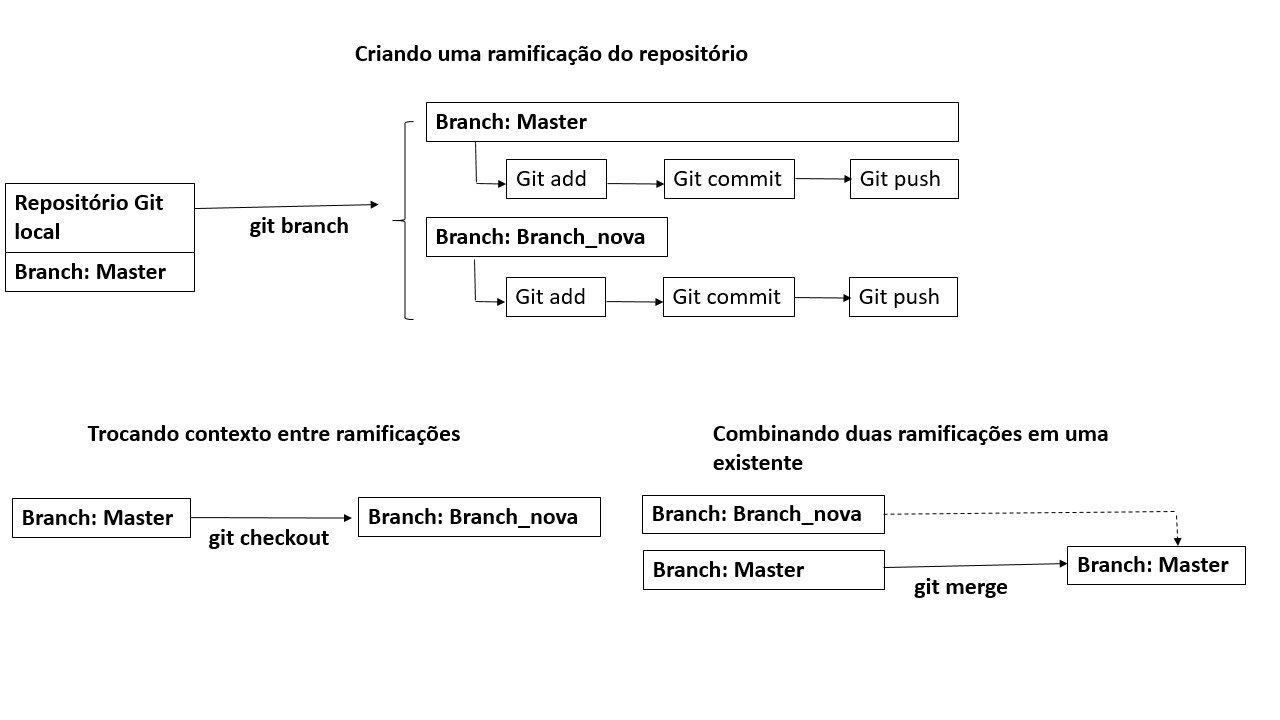
\includegraphics[scale=0.35]{img/git2.jpg}     
    \end{center}
}



\begin{frame}[fragile]  \frametitle{Conflito de Versões}
\begin{itemize}
      \IteOne{Conflitos são situações em que o git não consegue atualizar um arquivo com uma nova versão da branch automaticamente}
      \IteOne{Nesses casos o git avisa essa situação e pede para que o desenvolvedor resolva os conflitos}
\end{itemize}

Exemplo de conflito:
\begin{verbatim}
<<<<<<< branch1
#include "test.h"
 int main()
{
   return 0; 
} 
 ======= 
// needed a source code file 
>>>>>>> master 
\end{verbatim}
\end{frame}

\SliT{Github}{
\begin{center}
    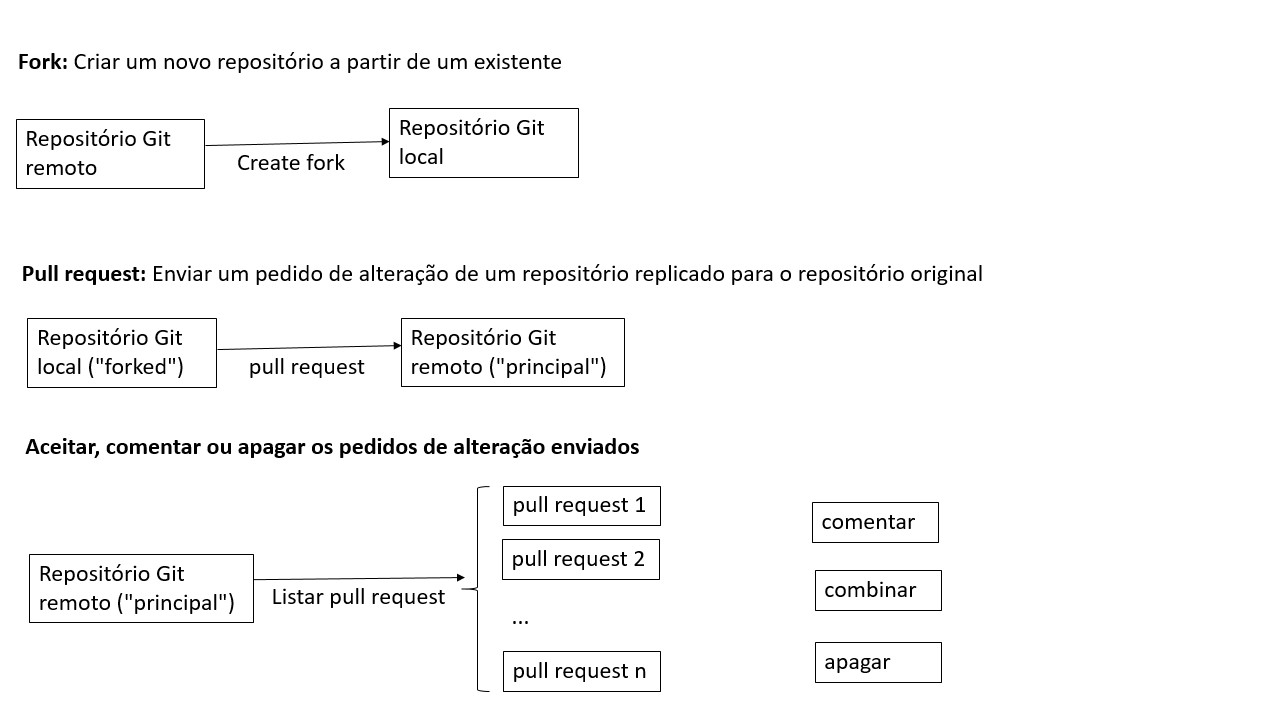
\includegraphics[scale=0.35]{img/git3.jpg}     
    \end{center}
}

\SliT{Github - Issue}{
\begin{center}
    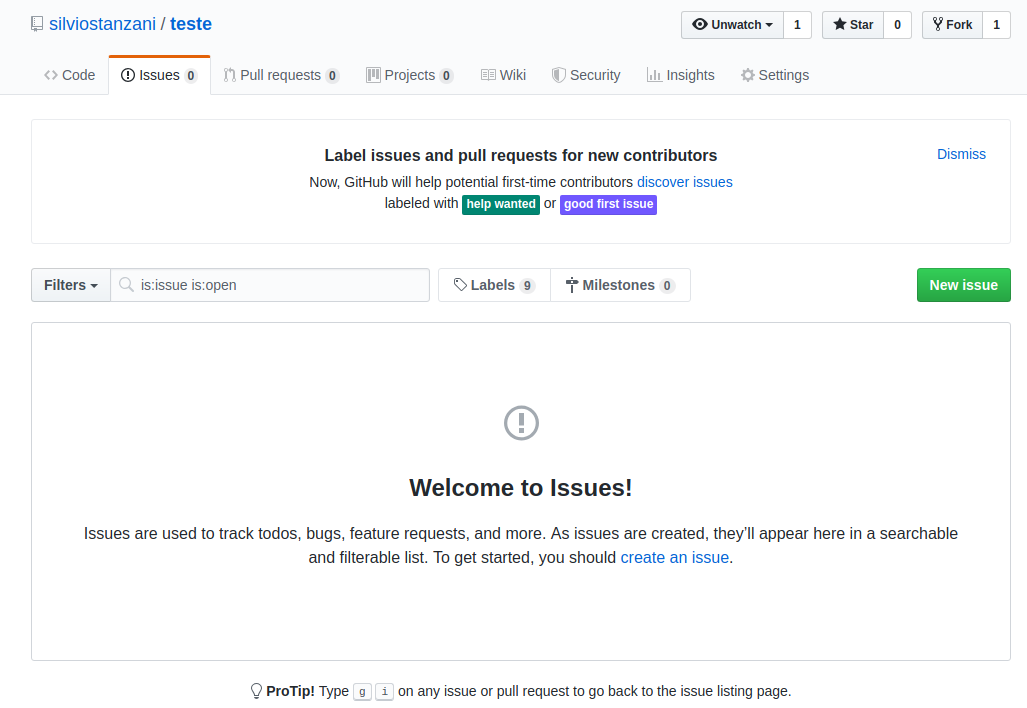
\includegraphics[scale=0.35]{img/issue.png}     
    \end{center}
}

\SliT{Github - Issue}{
\begin{center}
    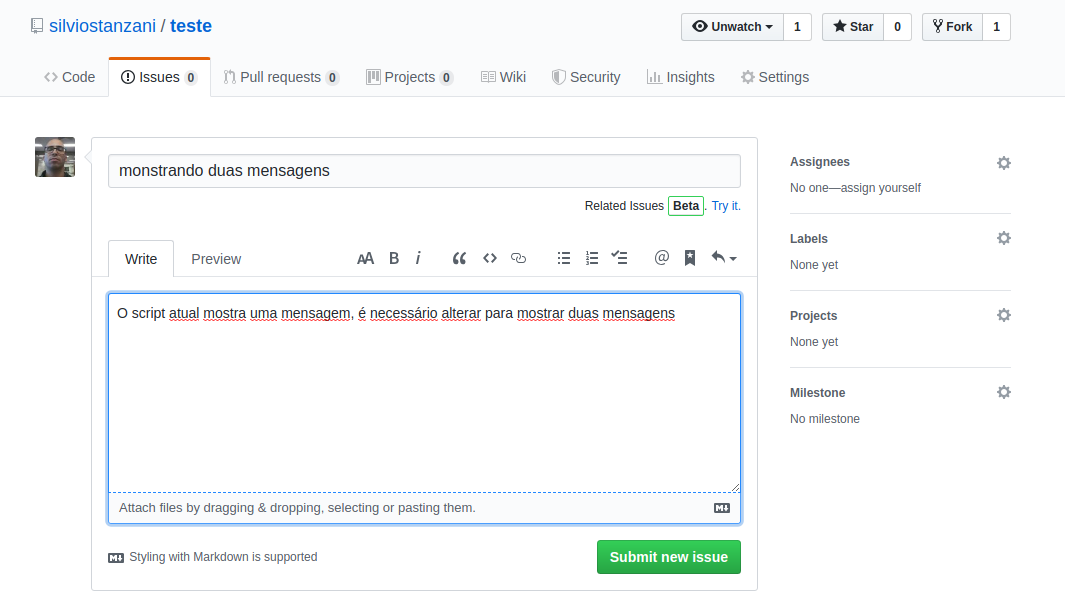
\includegraphics[scale=0.35]{img/issue2.png}     
    \end{center}
}

\SliT{Github - Issue}{
\begin{center}
    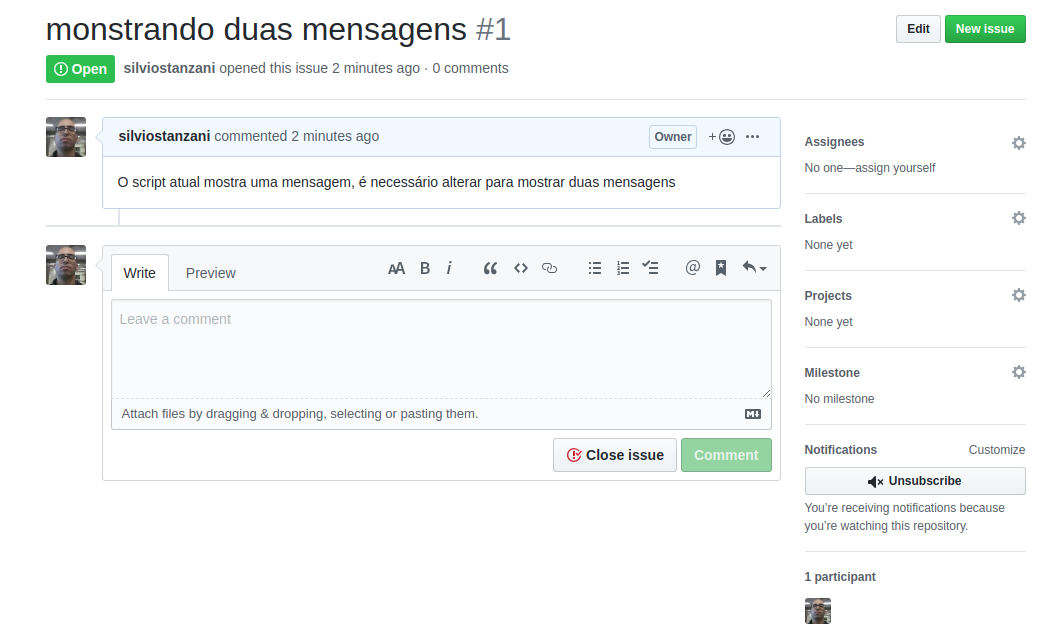
\includegraphics[scale=0.35]{img/issue3.png}     
    \end{center}
}

\SliT{Github - Fork}{
\begin{center}
    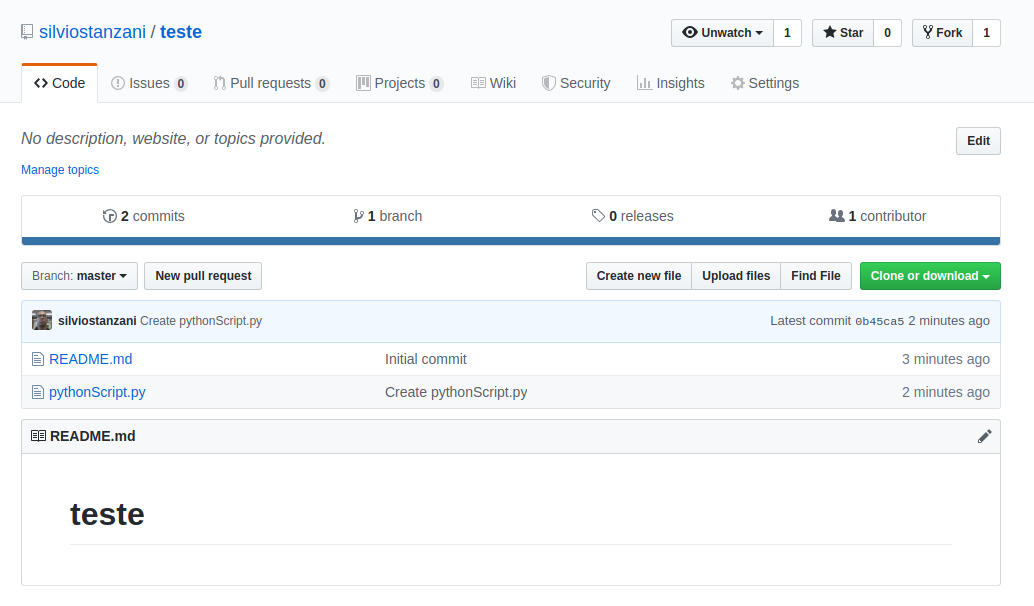
\includegraphics[scale=0.35]{img/mainrep.png}     
    \end{center}
}

\SliT{Github - Fork}{
\begin{center}
    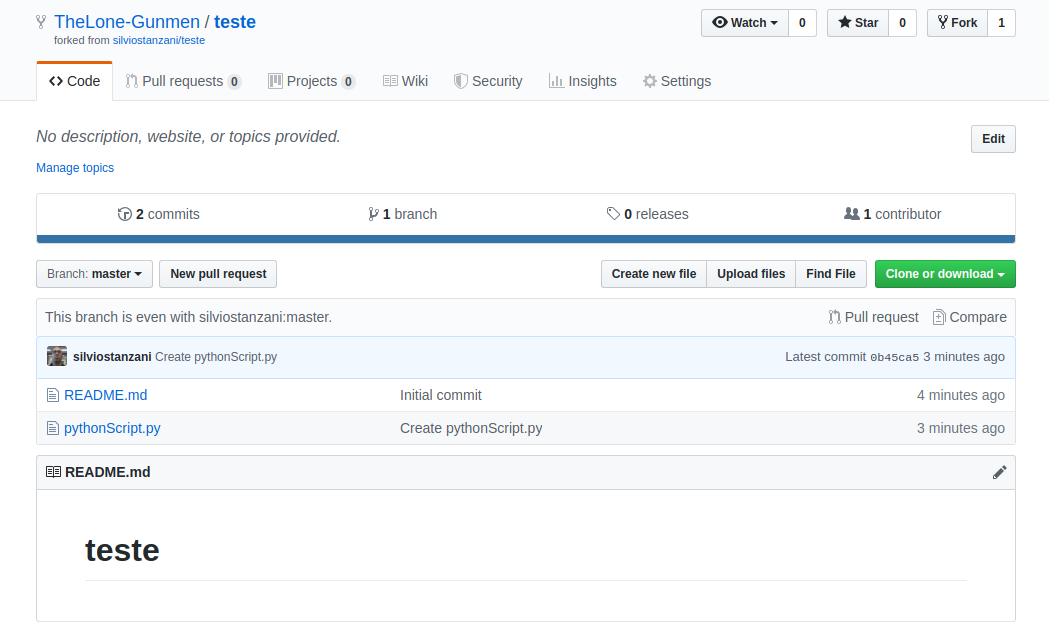
\includegraphics[scale=0.35]{img/main-forked.png}     
    \end{center}
}

\SliT{Github - Pull Request}{
\begin{center}
    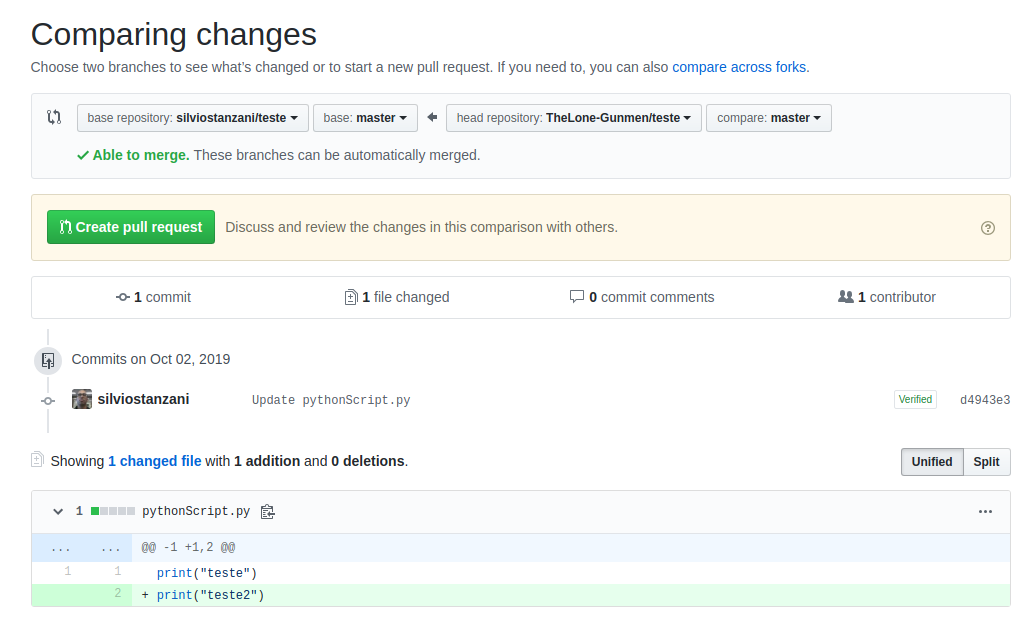
\includegraphics[scale=0.35]{img/pull-request.png}     
    \end{center}
}

\SliT{Github - Pull Request}{
\begin{center}
    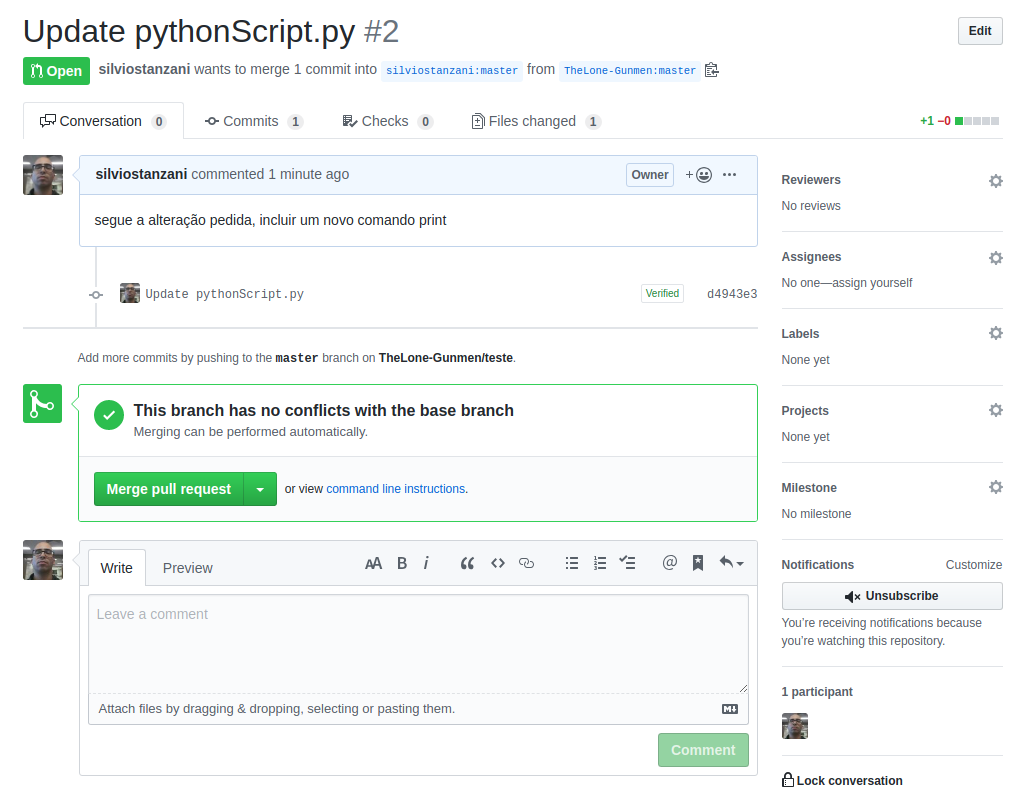
\includegraphics[scale=0.35]{img/pullre1.png}     
    \end{center}
}

\SliT{Referências}{

\begin{itemize}
    \IteOne{Site Git: http://git-scm.com/}
    \IteOne{Github : https://github.com}
    \IteOne{Materiais sobre git : https://try.github.io/}
    \IteOne{Na linha de comando: git help comando}
 \end{itemize}
}

% SLIDE NO TITLE
\Sli{
\secx{Dúvidas}
}

\end{document}
